\begin{frame}
  \frametitle{E -- Entertaining Excursion}
  \section*{Problem}
  Given a $NxM$ grid, find the number of ways $A \rightarrow B \rightarrow C$ such that no square is visited more than once.
\end{frame}
\begin{frame}
  \frametitle{E -- Entertaining Excursion}
  \section*{Solution}
  DP to rescue!

  There are sevelar cases to consider..
\end{frame}
\begin{frame}
  \frametitle{E -- Entertaining Excursion}
  \section*{Solution, Case 1}

  A C and B are on the same line.

  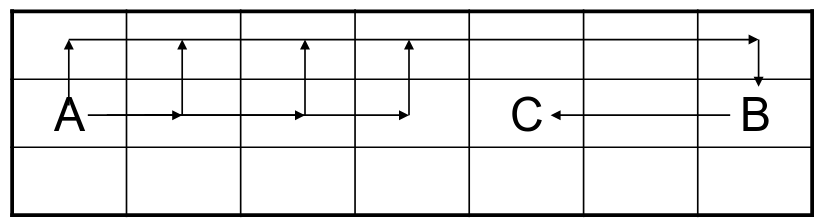
\includegraphics[height=3cm]{entertainingexcursion/case1.png}
\end{frame}
\begin{frame}
  \frametitle{E -- Entertaining Excursion}
  \section*{Solution, Case 2}

  B lies somewhere in between A and C.

  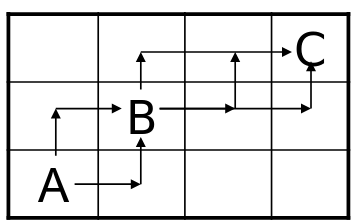
\includegraphics[height=3cm]{entertainingexcursion/case2.png}
\end{frame}
\begin{frame}
  \frametitle{E -- Entertaining Excursion}
  \section*{Solution, Case 3}

  B lies somewhere on the side of the line A and C.

  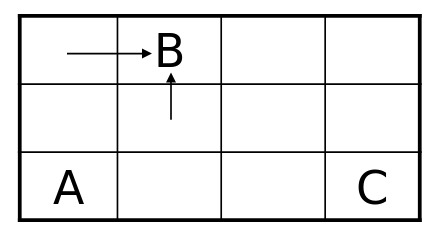
\includegraphics[height=3cm]{entertainingexcursion/case3.png}
\end{frame}

\begin{frame}
  \frametitle{E -- Entertaining Excursion}
  \section*{Solution, Case 3}

  Split it up in two subcases.

  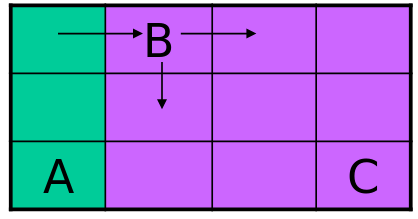
\includegraphics[height=3cm]{entertainingexcursion/case3_1.png}
  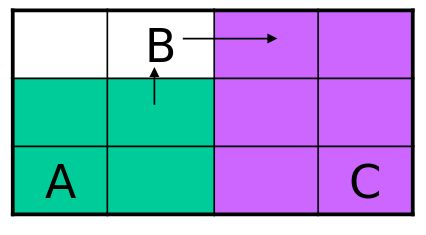
\includegraphics[height=3cm]{entertainingexcursion/case3_2.png}
\end{frame}
\begin{frame}
  \frametitle{E -- Entertaining Excursion}
  \section*{Solution, Case 4}

  B lies somewhere "on the corner" of A and C.

  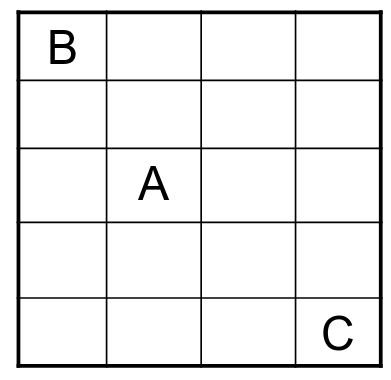
\includegraphics[height=3cm]{entertainingexcursion/case4.png}
\end{frame}
